\chapter{Ouverture à la concurrence des lignes de bus RATP et portabilité des droits à la retraite} % Main chapter title



Ma première tâche, en tant qu'alternant a porté sur les mécanismes de portabilité des droits à la retraite des agents RATP; aussi appelé le sac à dos social de la RATP.

Un sac à dos social est un dispositif qui a été créé lors de l'ouverture à la concurrence des services publics de transport ferroviaire de voyageurs. Le premier sac à dos social est à destination des salariés de la Société nationale des chemins de fer français (SNCF) qui ont été transférés à d'autres employeurs dans le cadre de l'ouverture à la concurrence.

Un sac à dos social est un accord qui définit, au-delà des règles déjà prévues par la loi (garanties de l’emploi et de rémunération, affiliation au régime spécial de retraite), les règles de transfert des garanties sociales dont ils bénéficiaient, telles que le maintien dans leur logement locatif, l’accès à la médecine de soins SNCF, la continuité des facilités de circulation, le devenir de leur compte-épargne temps, etc., chez leur nouvel employeur. 

L'ouverture à la concurrence du réseau historique de transport par autobus de l'Île-de-France est un projet initié par le droit européen et préparé par la législation française depuis plus de 15 ans. Ce projet implique également la mise en place d'un sac à dos social. Nous détaillerons dans cette partie les contributions des bureaux 3C et 3B à ce projet.

Une première partie sera consacré à présenter les origines de la réforme, le rôle de l'union Européenne etc. Une seconde partie exposera les spécificités du régime de retraite de la RATP par rapport au régime général. Enfin, la troisième partie me permettra d'exposer les spécificités du sac à dos social de la RATP et sa mise en place.



%----------------------------------------------------------------------------------------
%	SECTION 1
%----------------------------------------------------------------------------------------
\section{L'ouverture de la RATP à la concurrence et conformité au droit européen}

\subsection{La concurrence au niveau européen}


\begin{quote}
\begin{center}
\textit{``La solidarité de production [...] manifestera que toute guerre entre la France et l'Allemagne devient non seulement impensable, mais matériellement impossible.''}
\end{center}
\end{quote} \hfill Déclaration du 9 mai 1950, Robert Schuman

Cette citation est extraite de la déclaration ayant mené à la création de la Communauté européenne du charbon et de l'acier (CECA). Cette idée est présente depuis longtemps en économie :

\begin{quote}
\begin{center}
\textit{``Et c’est presque une règle générale, que partout où il y a des mœurs douces, il y a du commerce ; et que partout où il y a du commerce, il y a des mœurs douces''}
\end{center}
\end{quote} \hfill De l’esprit des lois, Chapitre XX (1748), Montesquieu

On peut résumer les résumer comme cela : "Il n y a qu'en ayant intégrant profondément les économies européennes entre elles qu'on évitera d'autres guerre." C'est dans ce principe que va se développer la Communauté Economique Européenne et le marché unique. 

Afin de permettre au marché unique de prospérer, l'Union Européenne s'est très rapidement emparée du sujet de la concurrence et en a fait une composante historique de sa construction. L'objectif est de se rapprocher de la concurrence pure et parfaite préconisée par les économistes néo-classiques. Pour cela il faut s'assurer que le marché est composé d’une pluralité d’acteurs (élimination des monopoles ou oligopoles) qui rivalisent sur des bases équitables afin qu'aucune entreprise ne puisse construire une position dominante et abuser de son pouvoir sur cet immense marché.

Ainsi dès 1957 et la rédaction du traité de Rome, aussi appelé traité sur le fonctionnement de l'Union européenne (TFUE), les états  confère une compétence exclusive à l’Union européenne en matière d’établissement des règles de concurrence. La politique de concurrence est ainsi mise en œuvre par des réglementations prises directement par la Commission européenne.



  \subsection{La concurrence au niveau des transports}

Afin de se rapprocher de la concurrence pure et parfaite entre les entreprises opérant sur le marché unique, et de respecter l'une de ses règles fondamentales, les différents membres de l'Union Européenne se sont accordé pour faire disparaître les derniers monopoles publics.
Dans cette partie, nous détaillerons la mise en oeuvre de ces accords dans le domaine des transports. En effet, ces services, dans l'Union Européenne, ont historiquement était gérés par des monopoles publics.

L'ouverture à la concurrence du rail européen a commencé en 2001 avec la publication des directives 2001/12/CE, 2001/13/CE et 2001/14/CE aussi appelées Premier Paquet Ferroviaire, qui ne concerne que le fret. 
Le deuxième paquet ferroviaire, adopté par la Commission européenne le 23 janvier 2002, a permis d'instaurer des règles d'interopérabilité et de fonctionnement ainsi que la création de l'Agence ferroviaire européenne.
C'est le troisième paquet ferroviaire, adopté en mars 2003, qu'est adopté l'ouverture à la concurrence les transports internationaux de passagers au sein de l'Union européenne.
Finalement, un quatrième paquet ferroviaire visant à ouvrir les lignes nationales et régionales commence à être étudié en 2013. Un accord n'est trouvé qu'en 2016. 

En France, c'est la SNCF qui est concerné par ces évolutions. Ci-dessous les dates importantes de l'ouverture à la concurrence des lignes SNCF.

\begin{figure}[htbp]
    \centering
    \includesvg[scale=0.85]{figures/chap1/concurrence-fr-1.svg}
    \caption{Calendrier d'ouverture à la concurrence des lignes SNCF}\label{fig:calsncf}
\end{figure}

Lors de l'ouverture à la concurrence d'un grand monopole, afin d'assurer une continuité des services, un processus de division en sous-lots et d'appel d'offre est organisé.

Imageons le processus avec l'exemple du train. Un sous-lots sera, par exemple, une liaison entre deux villes, par exemple le 'Lyon-Paris'. Une fois répartition en sous-lots faites, on réalise des appels d'offres sur ces liaisons. Un jury compare les propositions des différentes entreprises. Une fois qu'une entreprise candidate remporte un appel d'offre, les salariés du monopole publics travaillant sur cette liaison sont transférés dans l'entreprise vainqueur et continue de remplir les mêmes missions.

Ces transferts de salariés sont très importants pour garantir la continuité du service mais pose de nombreuses questions quand à leurs droits sociaux. En effet les monopoles publics français ont souvent des régimes de retraite, et de protection sociale plus généralement, qui sont spéciaux. Ils ont souvent des règles de cotisations et de liquidation très différentes du régime générale du privé. Or, les agents des monopoles, une fois transférés, sont soumis aux règles du régime générale. Les sac à dos sociaux permettent donc de gérer ces différences.


  \subsection{Ouverture de la concurence au niveau de la RATP}

  \subsubsection{Calendrier de la mise en oeuvre}

Suite à l'ouverture à la concurrence du réseau ferroviaire, c'est le réseau de transports en commun d'Île-de-France qui a du se mettre en règle vis à vis des règles concurrentielles de l'Union Européenne.
L'ouverture à la concurrence progressive des  transports en commun en Île-de-France a été encadrée par la loi n° 2009-1503 du 8 décembre 2009 relative à l’organisation et à la régulation des transports ferroviaires (ORT) de 2008. Mise en œuvre conformément au règlement européen du 23 octobre 2007, connu sous le nom de règlement OSP. Une date limite, fixée au 1er janvier 2025, avait été établie pour finaliser cette ouverture. Plus récemment, la loi d'orientation des mobilités (LOM) n° 2019-1428 du 24 décembre 2019 a déterminé le cadre social de la réforme.
C'est cette LOM qui a prévu, à l'article 158 un transfert automatique des contrats de travail des salariés de la RATP concourant à l’exploitation et à la continuité des services réguliers de transport public par autobus ou autocar. Ces transferts s’accompagne du maintien de garanties pour les salariés transférés.

Néanmoins, l'organisation des Jeux Olympiques et Paralympiques de Paris 2024 et les préoccupations liées à l'acceptabilité sociale du transfert de 19 000 salariés du réseau de bus de la RATP, dont environ 15 000 chauffeurs de bus, vers de nouveaux employeurs, nécessitent des ajustements spécifiques.

La Loi du 27 décembre 2023 relative à l'ouverture à la concurrence du réseau de bus francilien de la RATP permet à IDFM de décaler l'ouverture à la concurrence des bus franciliens sur une durée maximum de deux ans. Celle-ci devant intervenir entre le 31 décembre 2024 et le 31 décembre 2026. Il s'agit de faciliter et fluidifier l’ouverture effective à la concurrence.

Le calendrier ci-dessous a été établis en Janvier 2024 et avait pour objet de planifier les futurs tâches du bureau 3B permettant d'aboutir à la publication des décrets d'application de cette réforme. Il a été perturbé par la dissolution de l'Assemblée Nationale, rendant l'ensemble du gouvernement démissionnaire. Or c'est aux ministres et aux cabinets de trancher les décisions importantes, de prendre des arbitrages.

\begin{figure}[htbp]
    \centering
    \resizebox{\textwidth}{!}{
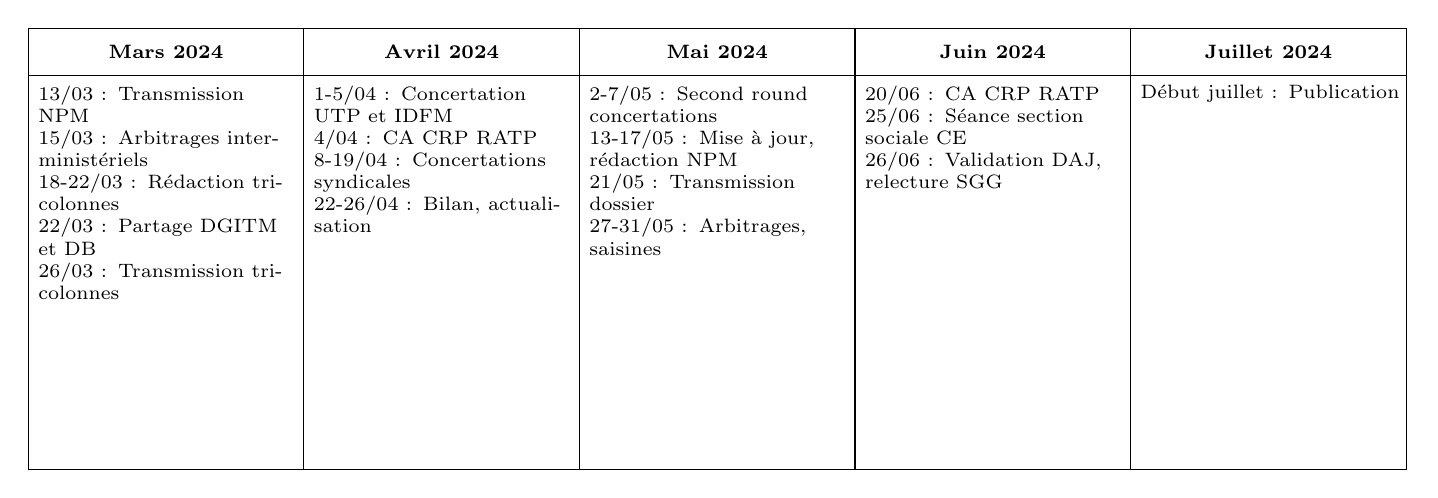
\begin{tikzpicture}[every node/.style={font=\scriptsize}]
\def\monthwidth{3.5cm}
\def\monthheight{5cm}
\def\headerheight{0.6cm}

% Macro for month column
\newcommand{\monthcolumn}[3]{
    % Header
    \draw (#1*\monthwidth,\monthheight) rectangle (#1*\monthwidth+\monthwidth,\monthheight+\headerheight);
    \node[anchor=center] at (#1*\monthwidth+0.5*\monthwidth,\monthheight+0.5*\headerheight) {\textbf{#2}};
    
    % Content
    \draw (#1*\monthwidth,0) rectangle (#1*\monthwidth+\monthwidth,\monthheight);
    \node[text width=3.3cm,anchor=north west,align=left] at (#1*\monthwidth+0.1,\monthheight-0.1) {#3};
}

% Mars 2024
\monthcolumn{0}{Mars 2024}{
    13/03 : Transmission NPM\\
    15/03 : Arbitrages interministériels\\
    18-22/03 : Rédaction tricolonnes\\
    22/03 : Partage DGITM et DB\\
    26/03 : Transmission tricolonnes
}

% Avril 2024
\monthcolumn{1}{Avril 2024}{
    1-5/04 : Concertation UTP et IDFM\\
    4/04 : CA CRP RATP\\
    8-19/04 : Concertations syndicales\\
    22-26/04 : Bilan, actualisation
}

% Mai 2024
\monthcolumn{2}{Mai 2024}{
    2-7/05 : Second round concertations\\
    13-17/05 : Mise à jour, rédaction NPM\\
    21/05 : Transmission dossier\\
    27-31/05 : Arbitrages, saisines
}

% Juin 2024
\monthcolumn{3}{Juin 2024}{
    20/06 : CA CRP RATP\\
    25/06 : Séance section sociale CE\\
    26/06 : Validation DAJ, relecture SGG
}

% Juillet 2024
\monthcolumn{4}{Juillet 2024}{
    Début juillet : Publication
}

\end{tikzpicture}
}
        \caption{Calendrier de travail du bureau 3B}\label{fig:retroplanning}
\end{figure}


  \subsubsection{Les enjeux de la réforme}

Pour le bureau 3B et 3C qui élabore cette réforme, les enjeux sont multiples :
\begin{itemize}
    \item Adapter la complexité du régime spécial de retraite afin de proposer un dispositif clair pour les nouveaux employeurs habitués au régime général.
    \item Éviter des effets gagnants/perdants parmi les salariés transférés.
    \item Rester en lien étroit avec les partenaires sociaux de la RATP pour s'assurer de l'acceptabilité sociale des mesures prises.
\end{itemize}

   
%----------------------------------------------------------------------------------------
%	SECTION 2
%----------------------------------------------------------------------------------------
\clearpage 

\section{Comparaison entre le regime spécial de la RATP et le regime général}

\subsection{Structure de l'emploi, de la rémunération et des droits associés}

Bien que les agents de la RATP soient des salariés de droit privé, ils sont néanmoins des salariés à statut. Cela ne signifie pas pour autant que ce sont des fonctionnaires.

Les explications que l'on trouve sur le site internet du Ministère de la Transition écologique et de la Cohésion des territoires sont particulièrement intéressantes :
\\
\textit{\\Ces statuts du personnel ont pour objet de prévoir notamment les conditions de recrutement et de cessation de fonctions, la rémunération, les congés de tout nature, certains droits syndicaux, les garanties disciplinaires. Ils sont élaborés au sein des établissements publics après consultation des organisations syndicales et font l’objet d’une approbation ministérielle. Ils revêtent la qualité d’actes réglementaires dont la légalité est soumise à l’appréciation du juge administratif.\\
Historiquement, la mise en place du statut dans les années 50 s’expliquait par la volonté d’exclure les entreprises publiques du champ de la négociation collective.
En vertu des dispositions de la loi du 11 février 1950 relative aux conventions collectives, les relations collectives de travail dans certaines entreprises et établissements du secteur public n’étaient pas déterminées par voie d’accord négocié, mais faisaient l’objet d’un statut législatif ou réglementaire. La loi fondait ainsi une exclusion réciproque entre accords collectifs et statuts de personnel.}

Ainsi, bien que les agents RATP ne soient pas des fonctionnaires, le fonctionnement de leurs rémunération s'inspire beaucoup de celui de la fonction publique.

Elle est composée d'un traitement indiciaire qui augmente avec l'ancienneté. Et de primes, qui elles sont versées en fonctions du travail ou des conditions de travail d'un agent. Il existe par exemple des primes de travail sur jours fériés, ou encore des primes pour conduite sans accident qui augmente avec le nombre de kilomètre parcouru sans accident.

Pour les salariés de droits communs, la rémunération est un salaire, encadré par les accords de branches. Il peut être négocié individuellement au moment de l'embauche. Une part du salaire peut également être variables et comprendre des primes.


\subsection{Assiette sociale et taux de cotisations}

Outre la structure des rémunérations, une des différences majeures entre le régime de la RATP et le régime générale se trouve au niveau des taux et assiettes de cotisations.
L'assiette de cotisation du régime spéciale de la RATP ne comprend pas l’ensemble des éléments de rémunération des salariés (en particulier, la plupart des primes). Alors que l'assiette de cotisation du RG comprend l'ensemble des éléments de rémunération.
Quant au taux de cotisation, il se décompose entre d’une part, le taux de cotisation salarial qui est supérieur à celui du régime général et s’établit à 12,95 \%, et d’autre part, le taux de cotisation patronal de 19,19 \% qui est révisé chaque année de telle sorte que la masse des cotisations soit équivalente à celle qui aurait été versée par l’employeur RATP si le régime avait été adossé au régime général. En pratique, le taux de cotisations à la charge de la Régie fait l’objet chaque année d’un arrêté fixant un taux de cotisations provisionnel pour l’année en cours qui devient définitif l’année suivante ; ce taux fait l’objet de régularisation afin de correspondre, en montant, à ce que la Régie aurait versé si ses salariés avaient relevé du régime général. Pour l’exercice 2022, le taux définitif de la cotisation à la charge de la RATP était fixé à 19,19 \%, tandis que le taux provisionnel de la cotisation à la charge de la RATP était fixé à 19,13 \% pour l’exercice 2023.  

Le calcul des droits à la retraite se fait également différemment. Comme pour les fonctionnaires, la pension à taux plein est égale à 75 \% du salaire (hors primes) des 6 derniers mois. Tandis que pour les salariés de droit communs la pension à taux plein est égale à 50 \% du salaire des 25 années les plus avantageuses de leurs carrière.


\subsection{Contrainte de la réforme : sauvegarde des droits futurs et de la rémunération}

En plus de toutes ces spécificités du régime de la RATP à prendre en compte lors du transfert des agents, l’article L. 3111-16-7 du code des transports a inscrit le principe d’une garantie de rémunération en cas de changement d’employeur des salariés RATP transférés dans le cadre de l’ouverture à la concurrence. Il est ainsi prévu que le niveau de rémunération des salariés transférés ne peut être inférieur au montant annuel, pour une durée de travail équivalente, des éléments de rémunération (traitement et primes), hors éléments exceptionnels, versés lors des douze mois précédant la date de changement effectif d’employeur. L’article précise que la garantie porte sur la rémunération nette de cotisations salariales. En pratique, le nouvel employeur verse au salarié une indemnité différentielle pour garantir son niveau de rémunération. Cette indemnité diminue en fonction des augmentations de salaire obtenues par le salarié après le transfert. En résumé, l'indemnité différentielle compense la perte de rémunération engendrée par le changement d’employeur.


%----------------------------------------------------------------------------------------
%	SECTION 3
%----------------------------------------------------------------------------------------
\clearpage 

\section{Mise en place du sac-à-dos Social}

\subsection{Alignement des cotisations pour les salariés transférés}

Afin de déterminer les taux et assiettes de cotisations applicables aux salariés transférés, deux scénarios ont été envisagés.
Soit l’application des taux et de l’assiette de cotisations sociales du régime général, soit le maintien des taux du régime spécial appliquée à une assiette de cotisations sociales reconstituée. Si ces scénarios sont neutres par construction pour la part patronale, leurs effets diffèrent sensiblement pour la part salariale. Pour le « sac à dos social » SNCF, l'option qui avait était privilégie était d’appliquer les taux de cotisations salarial et patronal du régime spécial de la SNCF aux salariés transférés et aux futurs employeurs sur la base d’une assiette de cotisations abattue afin de reconstituer l’assiette de cotisations du régime spécial.  

Dans le détail, le premier scénario consiste à appliquer les taux et l’assiette de cotisations salariale et patronale du régime général et du régime AGIRC-ARRCO sur la rémunération des salariés transférés. L’application des taux de droit commun présente une meilleure lisibilité et une simplicité de mise en œuvre pour les employeurs. Un seul système de cotisations existerait avec une implémentation facilitée, notamment d’un point de vue déclaratif dans les systèmes d’information (DSN notamment).
Ce scénario présente toutefois une difficulté juridique au regard du principe d’égalité devant les charges publiques. En effet, les salariés transférés continueront de bénéficier des pensions et prestations – modulo les adaptations nécessaires pour tenir compte du changement d’employeur – du régime spécial de retraite de la RATP tout en cotisant avec des taux différents de ceux des salariés statutaires. De plus ce scénario créerait de fortes distorsions entre les salariés compte tenu de la forte variabilité de
la part des éléments non-cotisables dans leur rémunération, rendant peu justifiable la dérogation au principe d’égalité devant les charges publiques. 

Par exemple, un cadre du réseau de surface transféré, dont la rémunération comporte peu de primes non cotisables, verserait moins de cotisations sociales (- 4 383 €) du fait de la baisse du taux de cotisations alors qu’un machiniste receveur de grade BC2, dont la rémunération statutaire est composée de nombreuses primes non cotisables, devrait cotiser après son transfert sur la totalité de sa rémunération (+ 5 652 €).

L’option alternative consisterait à maintenir les taux de cotisations sociales du régime spécial sur les rémunérations des salariés transférés.  L’application des taux de cotisations du régime spécial suppose de reconstituer l’assiette de cotisations sociales sur le modèle de l’assiette du régime spécial afin de reprendre la part des éléments cotisables et ceux non-cotisables dans la rémunération totale. 

Dans ce objectif, deux solutions ont été envisagées : 
\begin{itemize}
    \item application d’un coefficient d’abattement par groupements d’emplois : au moment du transfert, l’agent se verrait appliquer un coefficient d’abattement, défini en fonction de son emploi, sur sa rémunération. La liste des coefficients d’abattement serait définie par arrêté en fonction du type d’emploi, de sorte qu’en cas de changement d’emploi, le salarié se verrait appliquer un nouveau coefficient d’abattement pour la reconstitution de son assiette de cotisations ;
    \item exclusion de l’assiette de cotisations des éléments non cotisables : un arrêté fixerait la liste des éléments non cotisables (primes) en cohérence avec la structure de rémunération des salariés statutaires : l’assiette ainsi reconstituée serait individualisée et évolutive.
\end{itemize}

Pour la première solution, des coefficients d’abattement devraient être déterminés pour reconstituer l’assiette de cotisations. Le coefficient appliqué serait celui correspondant au métier exercé au moment du transfert, sans possibilité d’actualisation des coefficients car, contrairement au modèle SNCF, l’ensemble des métiers concernés par l’ouverture à la concurrence ont vocation à être transférés.

J'ai donc été chargé d'explorer les différentes manières de calculer un coefficient d'abattement permettant de reconstituer l'assiette de cotisation. C'est un travail de résolution d'équation qui fut long mais très intéressant et que je vais détailler ci dessous :


Pour commencer, mes variables sont : \\
Coefficient pour égaliser les assiettes : \(X\) \\
Rémunération RATP : \(Rem_{RATP} = RI + Primes\) \\
Cotisation RATP : \(Cotis_{RATP} = RI \times tx_{RATP}\) \\
Rémunération après transfert : \(Rem_{post-transfert}\) \\
Cotisation au RG : \(Cotis_{RG} = (RI + Primes) \times tx_{RG}\) \\
\\
On veut que la rémunération nette après transfert soit supérieure ou égale à la rémunération nette. \\
On a donc : 
\[
Rem_{post-transfert} - Cotis_{RG} \geq Rem_{RATP} - Cotis_{RATP}
\]
On pose notre équation comme suit : 
\begin{multline*}
Rem_{RATP} - (RI \times tx_{RATP}) = Rem_{post-transfert} \\
- (RI + Primes) \times tx_{RG} \times X \\
\end{multline*}
\text{Ici, les deux rémunérations s'annulent et on a donc :} \\
\begin{align*}
- RI \times tx_{RATP} &= - (RI + Primes) \times tx_{RG} \times X\\
X &= \frac{RI \times tx_{RATP}}{(RI + Primes) \times tx_{RG}} 
\end{align*}


Ce résultat est finalement assez intuitif. Le coefficient permettant de reconstruire l'assiette est le rapport des cotisations à la RATP sur les cotisations post-transfert. Ce coefficient permet d'égaliser parfaitement les rémunération avant et après transfert, mais pour des problématiques de système d'information, cette solution de coefficient individuel n'a pas pu être retenu. J'ai ensuite réaliser différents tests avec des coefficients moyen et médian par catégorie d'emploi mais les résultats n'ont pas été très satisfaisant. En effet les situations dans une catégorie d'emploi était trop variable et l'application de coefficient moyen ou médian créer de fortes inégalités.

Nous avons donc décidé d'abandonner cette piste. De plus, il était important que le coefficient et l'indemnité différentielle apparaissent tout deux dans l'équation. J'ai donc recommencer le travail avec ces deux inconnus. Je recommence donc le travail en posant l'équation comme cela :
\begin{equation*}
Rem_{RATP} - Cotis_{RATP} = Rem_{post-transfert} + ID - (X \times tx_{RG} \times (Assiette + ID))\\
\end{equation*}
\\
\text{Je ne détaillerais pas les calculs qui sont un peu longs mais on aboutit aux deux valeurs suivantes :} \\
\begin{multline*}
X = \frac{Cotis_{RATP}}{(Rem_{post-transfert} + ID) \times tx_{RATP}}\\
\\
ID = \frac{Cotis_{RATP}}{X \times tx_{RATP}} \min Rem_{post-transfert}
\end{multline*}


Ici, on aboutit à une solution ou le coefficient et l'indemnité différentielle sont inter dépendant. Si on veut augmenter l'indemnité différentielle jusqu'à un certain niveau, on doit également modifié X, ce qui fait baisser ID, on doit donc réaugmenter ID au niveau souhaitez etc.

Finalement ce scénario qui avait été retenu dans le cadre du sac à dos social SNCF, a été rejeté par la RATP dans la mesure  où la structure de rémunération de la RATP induit de fortes disparités entre agents appartenant à une même  catégorie d’emploi. En outre, contrairement à la branche ferroviaire, il ne sera pas possible de faire évoluer régulièrement le niveau des coefficients d’abattement dans la mesure où il  est prévu de transférer la quasi-intégralité des salariés de la RATP à terme.

Par conséquent, c'est le second scénario qui a été choisi. Il nécessite néanmoins de définir suffisamment précisément la  liste des éléments non cotisables afin de limiter le risque d’effet d’aubaine pour les employeurs qui pourraient être  incités à augmenter la part de ces éléments dans la rémunération pour réduire l’assiette cotisable. 

Concrètement, ce travail consiste à répertorier de manière exhaustive les primes RATP non cotisables que les salariés transférés auraient pu percevoir ou continuer à percevoir à l’EPIC en l’absence de transfert puis à transposer ces primes non cotisables en primes du droit commun, en leur attribuant une dénomination et des conditions d’obtention analogues et ne souffrant aucune ambiguïté.


\subsection{Avenir de la réforme}

L'arbitrage de Matignon sur le périmètre de transposition des primes ayant était rendu avant la dissolution, le travail de rédaction des textes juridiques a pu être finalisé cet été.
Une concertation avec les organisations syndicales, patronales, certaines entreprises candidates et la RATP a pu être menée.

Les premiers décrets ont pu être soumis au Conseil d'Etat fin août et les arrêtes sont eux en cours de validation en interne.

Cette mission a été très intéressante pour plusieurs raison. Elle m'a permit d'assister en direct à l'élaboration de mesures politiques particulièrement sensibles. J'ai pu travailler en collaboration avec un grand nombre d'acteurs institutionnels ou du secteur du transport. Cette mission m'a également permis de faire face aux difficultés inhérentes à ce type de travaux. De nombreuses possibilités doivent être explorées même si elles ne sont finalement pas adoptées. 

			%2 - Conclusion

%Gros travail sur le scénario avec détermination d'au taux

%#### Equation de détermination du coef d'abbatement

%####  Chiffagres individuels, par moy ou med de groupe
%- tableau resume pour NPM avec cas types

%#### difficulté juridique, on opte pour la ersion avec listes de primes

